\chapter{Introduction}
\label{cha:introduction}

This chapter introduces the thesis along with the concepts of allostery in proteins, structure-based allosteric prediction, normal mode analysis (NMA), the protein structural ensemble, protein kinases and cyclin-dependent kinase 2 (CDK2).
Further details on concepts and methods will be described in individual chapters as required.


\section{Overview of this thesis}
\label{sec:introduction_overview}

The aim of this thesis is to contribute to the field of allosteric site prediction by developing computational methods and testing them experimentally.
A summary of the concept of allostery in proteins and the recent emergence of approaches to predict allostery will be given.
The protein structural ensemble and methods to generate ensembles will be introduced.
Protein kinases are an important family of proteins that are amenable to allosteric regulation.
Protein kinases in general, and CDK2 in particular, will be described.

Chapters~\ref{cha:allopred} and \ref{cha:exprose} decribe two independent computational methods to predict allosteric sites on proteins, AlloPred and ExProSE.
AlloPred uses NMA and machine learning to rank pockets in terms of their allosteric character.
ExProSE uses distance geometry to generate structural ensembles that can be perturbed to explore dynamics and allostery.
The implications of each method are discussed in the respective chapters.

Chapter~\ref{cha:cdk2} describes the further testing of a potential allosteric site on CDK2 predicted as allosteric.
Virtual screening led to experimental assays being carried out on selected compounds.
Some conclusions are drawn in Chapter~\ref{cha:conclusion}.
Finally, Chapter~\ref{cha:appendices} contains the appendices.
The technical documentation for the AlloPred and ExProSE source codes is attached along with the description of a module to read, write and manipulate protein structure files in the Julia programming language.


\section{Allostery in proteins}
\label{sec:introduction_allostery}

Allostery in its broadest sense is the functional change at one site on a protein caused by a change at a distant site.
The perturbation at the allosteric site can be non-covalent binding of a molecule (e.g.\ small molecule, ions, RNA, DNA), covalent binding (e.g.\ phosphorylation) or light absorption \cite{Nussinov2013}.
Changes in structure or dynamics lead to effects such as a reduction or increase in catalytic activity, changes in disordered regions or changes in oligomerisation state.
All proteins are potentially allosteric \cite{Gunasekaran2004}.
This intrinsic and widespread property of proteins is important in processes such as cellular signalling and disease, yet most allosteric mechanisms remain an enigma and a universal mechanism has not been found \cite{Motlagh2014}.

Since the first discovery of allosteric systems more than 50 years ago there have been various models put forward to describe the phenomenon.
The dominant proposals for many years were the Monod-Wyman-Changeux (MWC) model, which posited that pre-existing states are subject to an equilibrium shift on modulator binding \cite{Monod1965}, and the Koshland-N\'{e}methy-Filmer (KNF) model, which advanced the idea that there was an induced fit of a binding site on interaction with a modulator \cite{Koshland1966}.
The structural view of allostery \cite{Perutz1970}, which aimed to elucidate the allosteric mechanism by finding structural changes on effector binding, began to fill the gaps left by the phenomenological MWC and KNF descriptions.
The discovery that entropic contributions to allostery can be significant predicted the phenomenon of allostery without conformational change \cite{Cooper1984}, where the allosteric effect is communicated by a change in protein dynamics rather than protein structure \cite{Motlagh2014}.

More recently these views on allostery have been revisited and reconciled in approaches that focus on the ensemble of conformational states that proteins exist in \cite{Motlagh2014, Hilser2012, Cui2008, Tsai2014}.
Figure~\ref{fig:allostery} outlines the current understanding of allostery.
A perturbation at any site in the structure leads to a shift in the occupancy of states by the population, so allostery is a property of the conformational ensemble.
The effect at the allosteric site is linked to the active site by small conformational changes that transmit the allosteric effect in a wave-like manner along pathways of amino acids in the protein \cite{DelSol2009}.
These pathways may be conserved by evolution \cite{Suel2003}.
It is also important to consider the effect of allostery on cellular networks and reaction pathways \cite{Nussinov2013}, with allosteric effects propagating via protein-protein interactions.

Allosteric drugs have hardly been explored and are a major avenue of research for the pharmaceutical industry \cite{Wenthur2014}.
They hold many potential benefits over orthosteric (non-allosteric) drugs: they do not bind to active sites that are often conserved in protein families, and are hence highly specific; they can activate as well as inhibit a protein; they can have a ceiling to their effect; and they can be used effectively in combination with orthosteric drugs \cite{Wenthur2014}.
The discovery of positive and negative allosteric modulators of GPCRs has highlighted these advantages \cite{Wootten2013, Conn2009}.
GPCR modulators include the positive regulator cinacalcet at the Ca\textsuperscript{2+}-sensing receptor and the negative modulator maraviroc of the chemokine CCR5 \cite{Nussinov2013}.
Allosteric modulators have been elucidated for targets as diverse as the GABA receptor, hepatitis C virus polymerase and RNA.
Numerous other allosteric modulators are in various stages of human clinical trails.
However, discovery of allosteric drugs presents challenges beyond those encountered in orthosteric drug discovery - see later.

In order to understand and utilise allostery it is necessary to be able to predict allosteric sites, allosteric modulators and residues involved in propagating the allosteric signal.
Advances from the last few years in the structure-based prediction of protein allostery are outlined here, largely focusing on computational approaches.
Review papers have covered similar topics \cite{SchuelerFurman2016, Wagner2016, Guarnera2016, Lu2014}.
The emerging fields of cryptic allosteric site discovery and allosteric site design are described and some of the issues surrounding allostery are discussed.


\begin{figure}
\centering

\includegraphics[width=0.9\textwidth]{figures/allostery/allostery}

\caption[The current conception of allostery as a property of the conformational ensemble]
{The current conception of allostery.
(A) A two-state model of allostery where a protein has an active and an inactive conformation.
In the presence of the allosteric inhibitor the inactive state is favoured either by the inhibitor binding to the protein when it is in the inactive state (red arrow - conformational selection) or by the inhibitor binding to the active state and causing inactivation (blue arrow - induced fit).
(B) The variety of motions that can lead to allostery.
Larger motions or more disorder are shown further down the vertical axis.
Figure based on Figure~2 from Motlagh et al.\ 2014 \cite{Motlagh2014}.
(C) A simplified representation of the change in the energy landscape on binding of an allosteric inhibitor.
The shaded regions show the main occupied conformation in each case.
On inhibitor binding the relative energies of the active and inactive states are altered.
For example, disruption of a hydrogen bond could destabilise the active state and stabilise the inactive state.
(D) Glucokinase, a well-studied example of allostery \cite{Kamata2004}, is shown as a yellow cartoon.
The glucose substrate and the allosteric modulator are shown as spheres coloured by element.
The active site and allosteric site are coloured purple and green respectively.}

\label{fig:allostery}
\end{figure}


\subsection{Computational methods for allosteric prediction}

The last few years have seen the emergence of the first general methods that predict allostery based on protein structure.
Table~\ref{tab:allosteric_methods} summarises these methods, many of which are available as web servers.


\begin{sidewaystable}
\centering

\begin{footnotesize}
\begin{tabular}{ l l p{5cm} l l }
\hline
Name & Reference(s) & Output(s) & Web server available & Source code available online \\
\hline
AlloPred & \cite{Greener2015} & Predicted allosteric pockets & \url{http://www.sbg.bio.ic.ac.uk/allopred/home} & Yes, MIT licence \\
AlloSigMA & \cite{Guarnera2017} & Allosteric free energies & \url{http://allosigma.bii.a-star.edu.sg/home} & No \\
AlloSite & \cite{Huang2013} & Predicted allosteric pockets & \url{http://mdl.shsmu.edu.cn/AST} & No \\ % AlloSitePro?
AllosMod & \cite{Weinkam2012} & Modelled energy landscapes & \url{http://modbase.compbio.ucsf.edu/allosmod} & No \\
ENM method & \cite{Li2017} & Residues coupled to normal modes & \url{http://enm.pitt.edu} & Partly as ProDy, MIT licence \\
ExProSE & \cite{Greener2017} & Ensemble of protein structures,\newline predicted allosteric pockets & No & Yes, MIT licence \\
MCPath & \cite{Kaya2013} & Allosteric communication pathways & \url{http://safir.prc.boun.edu.tr/clbet_server} & No \\
PARS & \cite{Panjkovich2014, Panjkovich2012} & Predicted allosteric pockets & \url{http://bioinf.uab.cat/pars} & No \\
SPACER & \cite{Goncearenco2013, Mitternacht2011} & Predicted allosteric residues,\newline exploration of allosteric communication & \url{http://allostery.bii.a-star.edu.sg} & No \\
STRESS & \cite{Clarke2016} & Predicted surface-critical and interior-critical residues & No & Yes \\
\hline
\end{tabular}
\end{footnotesize}

\caption[Computational allosteric prediction methods currently available to run locally or as a web server]
{Computational allosteric prediction methods currently available to run locally or as a web server, ordered alphabetically.
The work presented in this thesis (AlloPred and ExProSE) is included.
In addition there are various pocket prediction methods that aim to predict binding pockets on proteins, but not specifically allosteric pockets \cite{Huang2006, LeGuilloux2009, Cimermancic2016}.}

\label{tab:allosteric_methods}
\end{sidewaystable}


\subsubsection{Normal mode analysis}

In NMA the structural fluctuations of a protein around an equilibrium conformation are decomposed into harmonic orthogonal modes \cite{Hayward2008}.
Each mode has all parts of the system moving sinusoidally, in phase and with the same frequency.
All observed configurations of the system can be generated from a linear combination of its normal modes.
The process of NMA is shown in Figure~\ref{fig:nma}.
The normal modes are found by diagonalising the Hessian matrix - the matrix of second derivatives of the potential energy with respect to the mass-weighted atomic coordinates.
NMA is effective at describing protein dynamics, despite ignoring the complex nature of the protein energy landscape \cite{Bahar2005}.
Even considering the C\textsuperscript{\textalpha} atoms alone as a network of balls and springs can be sufficient, meaning that NMA is a computationally efficient way of exploring protein flexibility compared to molecular dynamics (MD).
This simplification is called the elastic network model (ENM) and the mathematical formulation is described in Section~\ref{sec:allopred_methods}.
The long-range nature of allosteric communication is often well-described by low-frequency modes that involve the motion of many atoms.
However, allostery does involve local effects so higher-frequency modes should also be taken into account \cite{Collier2013}.

The binding leverage approach \cite{Mitternacht2011} predicts how ligand binding couples to the intrinsic motions of a protein.
Sites with high binding leverage are predicted to be allosteric.
Binding leverage was developed into the web server SPACER \cite{Goncearenco2013}, and into the general predictor STRESS \cite{Clarke2016} by a different group.
% Mention other Mitternacht methods? Geometry/local closeness
% This has been further developed \cite{Guarnera2016a}...
% And turned into a web server \cite{Guarnera2017}...
The PARS method \cite{Panjkovich2012, Panjkovich2014} calculates normal modes in the presence and absence of a simulated allosteric modulator.
If the motions are significantly different the site is predicted as allosteric.
The DynOmics ENM server \cite{Li2017} finds hinge residues that control the two slowest normal modes of a protein, and hence are able to influence its dynamics.
Several studies have used NMA to model allosteric regulation in specific sets of proteins \cite{Balabin2009, Rodgers2013, Zheng2007, Su2014}.
NMA is suitable for high-throughput, automated approaches as it can be computationally inexpensive.
However whilst NMA-based methods might be expected to reveal perturbations to vibrations, the assumption of harmonic fluctuations around an energetically-minimum structure means that other contributing motions to allostery such as local unfolding and rigid body movements \cite{Motlagh2014} are not taken into account.


\begin{figure}
\centering

\includegraphics[width=\textwidth]{figures/nma/nma}

\caption[Steps in normal mode analysis]
{Steps in NMA using the ENM.
A protein structure is converted into an elastic network where balls are C\textsuperscript{\textalpha} atoms and springs are between C\textsuperscript{\textalpha} atoms within a certain distance.
A Hessian matrix of second derivatives of the potential energy $V$ in terms of the mass-weighted atomic coordinates $q_{i}$ is derived from the potential energy function of this elastic network.
Diagonalising the Hessian matrix yields eigenvectors and eigenvalues that correspond to the displacements for each C\textsuperscript{\textalpha} atom in a mode and the square of the mode frequency respectively.
See \cite{Hayward2008} for more.}

\label{fig:nma}
\end{figure}


\subsubsection{Machine learning}

A few methods have used machine learning to predict allostery.
AlloSite \cite{Huang2013} uses a support vector machine (SVM) and features from Fpocket \cite{LeGuilloux2009} to re-rank pockets in terms of their allosteric character.
However the results are often found to be similar to the Fpocket ranking, showing the difficulty of distinguishing pockets that have specific allosteric character from those that are generally suitable for ligand binding.
This method has been updated as AlloSitePro to include NMA perturbation \cite{Song2017}.
A Random Forest approach \cite{Chen2016} uses descriptors for binding sites and associated ligands to assign protein cavities as allosteric, regular or orthosteric.


\subsubsection{Molecular dynamics}

MD remains the standard computational tool for structural analysis when structures are available.
A study on the signaling protein NtrC combined MD simulations and NMR data to explore the free energy landscape and investigate at atomic resolution the transition from active to inactive state \cite{Pontiggia2015}.
% And Laine2010
Perturbation response scanning (PRS), in which the response of the structure to random perturbations at specific positions is examined, is a popular tool for allosteric prediction.
For example, allosteric hotspot residues were predicted using PRS for the chaperone Hsp70 \cite{Penkler2017}.
Weinkam et al.\ constructed energy landscapes and explored them with MD \cite{Weinkam2012}.
They were able to study the allosteric mechanisms involved in three proteins.
The method is available as the AllosMod web server.


\subsubsection{Evolutionary methods}

Classic work has shown that allosteric communication can be mediated by networks of residues conserved by evolution \cite{Lockless1999, Suel2003}.
One study developed previous work on protein sectors, groups of co-evolving residues physically contiguous in structure, to link sector-connected surface sites to allosteric sites \cite{Reynolds2011}.
A recent approach found that surface and interior critical residues tend to be conserved \cite{Clarke2016}.
The recent discovery that most directly co-evolving residues distant in 3D structure are close in related structures or assemblies \cite{Anishchenko2017} brings into question the concept of allosteric and active sites that directly co-evolve.
Other studies have found structural conservation in allosteric pockets but a lack of sequence conservation \cite{Panjkovich2010, Panjkovich2013}, positing that allostery makes use of pre-existing features.
As more structural and conservation information is acquired it will be important to discover to what degree allostery in proteins is a result of selection on specific pathways, and to what degree novel allostery can be discovered on proteins in the absence of previous evolutionary pressure.
% Be clear difference between conservation and co-evolution


\subsubsection{Other methods}

A recent study \cite{Amor2016} constructs an all-atom graph and calculates for each bond the bond propensity, the strength of coupling to the active site through the graph.
The method is used to reproduce observed results for three proteins in detail and is also able to predict allosteric sites in a dataset of 20 allosteric proteins.
Coarse-grained simulation approaches such as a two-state G\={o} model have also been utilised.
In one approach an ensemble of structures is generated and the response of the ensemble distribution to an effector is used to predict allostery \cite{Qi2012}.


\subsubsection{Methods not specific to allostery}

The identification of binding sites on the protein surface is a problem that has long pre-dated the search for pockets that are specifically allosteric.
These methods are however useful in the structure-based prediction of allostery - the identification of a high-affinity binding site distant from a known active site could present an opportunity for allosteric regulation, for example.
The FTMap family of web servers \cite{Kozakov2015} predicts ligand-binding hotspots using small organic molecules as probes on the protein surface.
By using mixed-solvent MD this principle has been extended to the prediction of allosteric sites in particular, with success on some test cases \cite{Ghanakota2016}.

Common pocket prediction methods such as LIGSITE\textsuperscript{\it csc} \cite{Huang2006} and Fpocket \cite{LeGuilloux2009} are able to find pockets on a protein large enough to bind small molecules, and these often correspond to allosteric sites \cite{Huang2013}.
These methods will be used throughout this thesis, and their ability to predict allosteric pockets (either alone or when re-ranked by allosteric prediction methods) will be determined.
Fpocket uses the concepts of Voronoi tessellation and alpha spheres (spheres touching four atoms at an equal distance) to find clusters of spheres of a certain size that correspond to pockets.
LIGSITE\textsuperscript{\it csc} adds the concept of conservation of surface residues to the original LIGSITE algorithm \cite{Hendlich1997}, which finds cavities using simple operations on a cubic grid.


\subsubsection{Allosteric pathway prediction}

Allosteric signals can be propagated by multiple communication pathways \cite{DelSol2009}.
Understanding these pathways is necessary in order to predict sites that are able to communicate with the active site \cite{Dokholyan2016}.
A machine learning approach to predict residues involved in allosteric communication uses a variety of structural and network features and is able to predict these hotspots with reasonable accuracy \cite{Demerdash2009}.
A different approach, McPath, uses a Monte Carlo algorithm to define likely allosteric pathways by examining inter-residue interactions in a residue network \cite{Kaya2013}.
A study that added an allosteric domain to a protein analysed residue contact maps to find loops mechanically-coupled to the active site \cite{Dagliyan2016}.
An investigation on the PDZ domain using MD found that allosteric changes are non-linear and occur in a non-local fashion, and are similar in many ways to protein folding \cite{Buchenberg2017}.
This study highlights that the idea of a single set of connected residues transmitting the allosteric signal is not adequate to explain allosteric communication.
In multimeric proteins it has been suggested that `global communication networks' of quaternary and tertiary motions transmit allosteric signals, and that considering these motions separately is inadequate \cite{Daily2009}.
Successful frameworks for predicting allosteric communication should take this into account.


\subsection{Experimental methods for allosteric prediction}

Experimental studies such as crystallography, NMR and site-directed mutagenesis remain the best tools for exploring allostery in a particular protein.
A synthetic azetidine derivative that kills Mycobacterium tuberculosis through allosteric inhibition of tryptophan synthase (TrpAB), a previously untargeted enzyme, was found by a high-throughput screen \cite{Wellington2017}.
The inhibition is not easily overcome by changes in metabolic environment due to the modulator binding at the TrpAB \textalpha -\textbeta -subunit interface and affecting multiple steps in the overall reaction of the enzyme.
A study on the proteasome \cite{Haselbach2017} crystallised the complex in the presence and absence of an allosteric modulator.
Having the active and inactive structures allowed the authors to propose a detailed mechanism of inactivation, which has implications for future allosteric proteasome inhibitors.
A study on flavovirus protease \cite{Brecher2017} used a virtual screen to select 29 potential allosteric compounds that were tested experimentally.
One showed an ability to inhibit the conformational change and also inhibit flavovirus growth.
Allosteric pathways in ERG proteins were proposed using fluctuation correlation data and validated by mutating residues in the pathways \cite{Ye2017}.
However, there are limits to the use of mutational studies to validate allosteric mechanisms.
It has been found that mutational data can give evidence for a deliberately poorly-conceived allosteric mechanism \cite{Tang2017}.
In the future it is to be hoped that experimental screens specifically for allosteric sites \cite{Martin2012, Jayakar2017, Pellerano2017, Pisco2017, Raman2014} become more widespread, opening the path to conventional large-scale screens for allosteric drugs.
% http://www.jbc.org/content/292/15/6429.full.pdf+html "Allostery modulates the beat rate of a cardiac pacemaker" NMR used
% Dror 2013 "Structural basis for modulation of a G-protein-coupled receptor by allosteric drugs" - actually this could go in MD section with a reference to long MD becoming more feasible
% https://www.nature.com/nsmb/journal/vaop/ncurrent/pdf/nsmb.3440.pdf - An information theoretic framework reveals a tunable allosteric network in group II chaperonins - could go in evolution section
% Shen2017 genomic screen


\subsection{Cryptic allosteric sites}

The discovery of cryptic binding pockets - pockets that are only available in some conformations of the protein and may not have an associated experimental structure - has the potential to vastly increase the number of druggable sites on proteins \cite{Boehr2009} and is directly relevant to allosteric prediction.
A recent study \cite{Lee2016} showed using NMR data that ligands of the LpxC enzyme access a cryptic site that is invisible to crystallography.
One study used Markov state modelling and MD to predict multiple hidden allosteric sites on \textbeta -lactamase and tested these using thiol labelling experiments \cite{Bowman2015}, later finding modulators for the sites \cite{Hart2017}.

The general approach CryptoSite uses machine learning to predict cryptic pockets on proteins using sequence and structural features \cite{Cimermancic2016}.
However, two problems affect the use of cryptic allosteric pockets over allosteric sites where the pocket is present in most or all conformations.
Firstly, the shape of the pocket is not known so rational drug design is difficult.
Secondly, there is potentially an energetic cost associated with the protein adopting the conformation required for the cryptic pocket \cite{Oleinikovas2016}.
However, the discovery of ligands with inhibition constants in the low picomolar range in the above study \cite{Lee2016} show that these sites are druggable.
Further computational and experimental studies are required to explore this promising area.


\subsection{Design of allosteric sites}

The rational design of allosteric sites is a problem closely related to structure-based prediction of allostery.
Introducing allosteric sites into existing proteins, or creating fusion proteins to add activity switches, has many potential applications including in biotechnology \cite{Makhlynets2015}.
A recent study added a PDZ domain into the Cas9 protein at a site that did not disrupt enzyme action \cite{Oakes2016}.
The protein showed modulator-dependent activity in cells, establishing a system for Cas9 activation.

Another study created fusion proteins that use conformational entropy to respond to temperature or pH as a switch \cite{Choi2015}.
Taylor et al.\ engineered \textit{E.\ coli} LacI to respond to one of four new inducer molecules using computational design and mutagenesis \cite{Taylor2016}.
Dagliyan et al.\ designed a protein with a unique topology, uniRapR, whose conformation is controlled by the binding of a small molecule \cite{Dagliyan2013}.
The switching and control ability of uniRapR was confirmed in silico, in vitro, and in vivo.
uniRapR was used as an artificial regulatory domain to control activity of kinases as a proof of concept.
The same group built on this and inserted the light-sensitive LOV2 domain into 3 proteins at non-conserved, surface-exposed loops identified computationally using residue contact analysis as being allosterically coupled to active sites \cite{Dagliyan2016}.


\subsection{Discussion of allostery}

It is challenging to compare different methods for allosteric prediction.
The different inputs and, more commonly, outputs make systematic comparisons difficult.
One of the Critical Assessment of Genome Interpretation challenges in 2015-16 focused on predicting the influence of mutations on the allosteric regulation of human liver pyruvate kinase \cite{Xu2017}.
However the uptake was limited to four groups and the predictive ability was marginally better than random.
In the long run a dedicated community-wide initiative similar to the Critical Assessment of Structure Prediction \cite{Moult2016} would be beneficial to the field of allosteric prediction.

One factor holding allosteric prediction back is the lack of a varied and robust set of benchmarks to test methods against.
ASBench \cite{Huang2015} is a curated set of allosteric proteins, and has been used for example to benchmark the method presented in Chapter~\ref{cha:allopred}.
It is a subset of the AlloSteric Database (ASD, \url{http://mdl.shsmu.edu.cn/ASD}) \cite{Shen2016}, which was set up in 2011.
ASD v3.0 contains over 1,400 proteins and 70,000 modulators and also includes allosteric mechanisms, allosteric networks of proteins and `allosteromes' of the allostery involved in protein kinases and GPCRs.
The allosteric proteins in the ASD are those that have experimental evidence for allostery.
The increasing number of entries in this database shows that a large number of proteins have allosteric character, and implies that many proteins have allosteric character yet to be discovered.
Improvements in such resources are necessary to prevent the developers of new methods having to assemble their own datasets \cite{Panjkovich2012, Mitternacht2011, Amor2016} and to allow systematic comparisons between methods.

An issue that requires more study in the field of allosteric prediction is the exact relationship between an allosteric modulator and whether it acts as an activator or inhibitor.
It has been shown that under different conditions the same allosteric modulator can have opposite effects \cite{Motlagh2012}.
Another viewpoint is the anchor/driver model of allostery, with the concept of a pushing or pulling driver determining which way the ligand acts \cite{Nussinov2014}.
An approach to study this would be a quantitative structure activity relation-like study where a variety of modulators and conditions are explored on the same protein.
This would give evidence as to whether small structural differences causing a pushing or pulling effect are enough to reliably switch activator/inhibitor action.

The mechanism of dynamic allostery, where the allosteric effect is transmitted through changes in dynamics and the average structure does not necessarily change, also requires further investigation.
While experimental studies \cite{Popovych2006, Capdevila2017, Wellington2017} have found evidence for dynamic allostery, Nussinov and Tsai \cite{Nussinov2015} warn that an apparent lack of conformational change can be an artefact of various factors such as crystal packing, crystallisation conditions, disorder to order transitions, incremental activation, synergy between allosteric sites and changes in oligomeric state.
A recent MD study proposes that allostery in the well-studied PDZ domain is driven by changes in electrostatic effects rather than solely changes in dynamics \cite{Kumawat2017, Liu2017}.
The role of water in allostery also needs to be further explored as evidence has been found that re-arrangement of water molecules is a possible mechanism of allostery \cite{Buchli2013, Amor2016}.
Studies that combine experimental and computational approaches \cite{Haselbach2017, Ozorowski2017} are well-suited to eploring these issues.


\subsection{Challenges in allosteric prediction}

There are a number of challenges faced in the structure-based prediction of protein allostery:

\begin{enumerate}
\item As shown in Figure 1B, an allosteric effect can arise from a variety of different mechanisms.
A general predictor would have to account for these in a unified manner.
This is particularly challenging when disorder is involved, as approaches based on a defined structure are less applicable.
Some approaches to studying disorder and allostery have been proposed \cite{Singh2017, Wang2017}.
\item The conformational changes that cause allostery are often large enough to occur on timescales of microseconds or milliseconds.
This makes them too computationally expensive to study using MD without the use of accelerated or targeted MD.
NMA is more computationally feasible but the assumption of a harmonic motion around an energy minimum does not correspond well to two distinct states with differing conformations.
\item The properties of active site pockets and small molecules that target the active site have been well-studied, for example Lipinski's rule of five \cite{Lipinski2001}.
Allosteric pockets and modulators may have generally different properties that we are not yet fully aware of, so we do not know exactly what to look for \cite{VanWesten2014, Wang2012}.
\item The effect of an allosteric modulator is difficult to predict and can range from activation to inhibition, partial or complete.
This is in comparison to orthosteric drug discovery, where drug action is presumed to be by competitive inhibition at the active site.
\item The effort of researchers and the protein structural data available is biased towards certain types of protein, such as those relevant in disease.
For example, the allostery of GPCRs has been studied in detail \cite{Wootten2013, Conn2009}.
There is a lack of protein structural data for important types of proteins such as membrane proteins and proteins with significant disorder, but these proteins have considerable potential to be allosteric \cite{Motlagh2014}.
There may be different mechanisms or approaches to prediction that are relevant to less-studied protein families.
The development of experimental methods such as cryo-electron microscopy should go some way to resolve this discrepancy \cite{Ozorowski2017}.
\end{enumerate}


\section{Protein structural ensembles}
\label{sec:introduction_ensembles}

% Expand NMR ensemble stuff
% FIRST, FRODA etc

Proteins move on a variety of timescales, encompassing motions from the vibration of a single bond to the collective movement of whole domains \cite{Henzler-Wildman2007, Wei2016} - see Figure~\ref{fig:timescales}.
X-ray crystallography provides a static view of the structure of proteins.
However, when only static structures are available the dynamic processes crucial to protein function \cite{Henzler-Wildman2007a} are hard to elucidate.
Experimental techniques to explore the dynamics of proteins, such as nuclear magnetic resonance (NMR) \cite{Sormanni2017}, are sophisticated and time-consuming.
Significant effort has gone into determining the protein structural ensemble when experimental data is available \cite{Bonomi2017}, but ideally there would be computational methods that worked in the absence of this information.

MD is a widespread computational method for predicting protein motions and generating ensembles of protein structures.
It is effective at modelling motions up to the timescale of nanoseconds.
However, the computational cost of modelling proteins on the scale of microseconds or milliseconds means MD is not suitable for larger-scale transitions.
Advanced MD methods such as targeted or accelerated MD can overcome this sampling problem \cite{Maximova2016}, but these methods are not yet routinely applicable due to the parameterisation and analysis required for each protein.


\begin{figure}
\centering

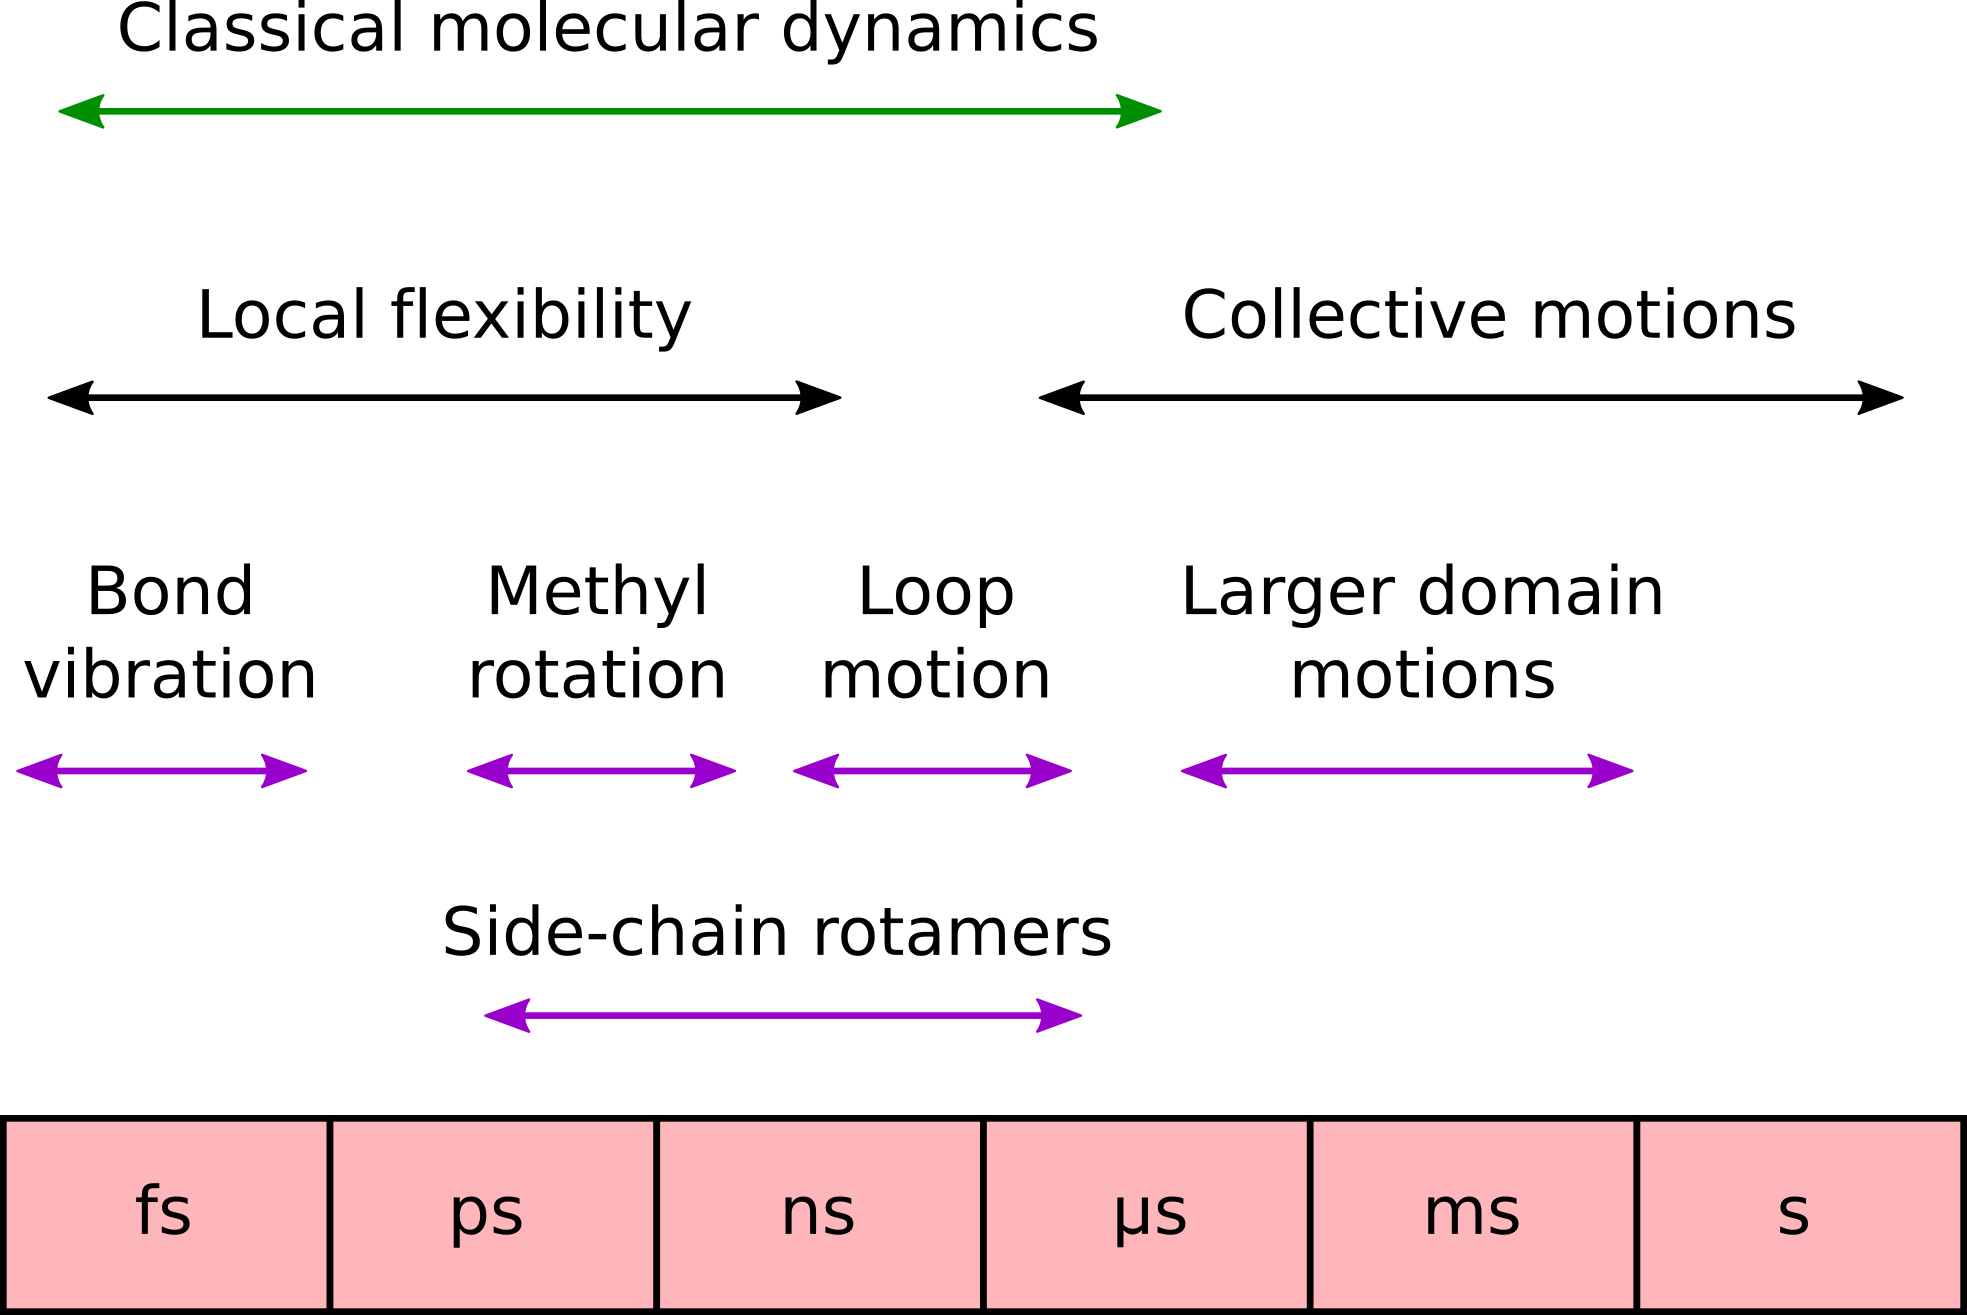
\includegraphics[width=0.7\textwidth]{figures/timescales/timescales}

\caption[Timescales of protein motions]
{Dynamic processes in proteins and their associated timescales.
Also shown is the range of timescales that can be studied with classical MD.
Figure based on Figure~1 from Henzler-Wildman and Kern 2007 \cite{Henzler-Wildman2007}.}

\label{fig:timescales}
\end{figure}


Various non-MD methods have been used to generate ensembles of protein structures from a crystal input structure, and hence explore protein dynamics.
CONCOORD \cite{DeGroot1997, DeGroot1999} is a distance geometry method to generate structures from an input structure and consists of a two-step process.
First, the different types of chemical interactions in the input structure, e.g.\ H-bonding and hydrophobic interactions, are converted to distance constraints with a given tolerance.
Next, an iterative minimisation procedure is performed to move a set of randomly-placed coordinates such that most distance constraints are satisfied.
This generates a protein structure in a similar manner to the way a structure is produced from NMR constraints.
The process is repeated to obtain an ensemble of structures.
tCONCOORD extends CONCOORD and gives better sampling of proteins with large conformational changes by predicting H-bonds in the structure that are liable to break \cite{Seeliger2007}.

NMA is also well-suited to studying flexibility and conformational change in proteins \cite{Dobbins2008}, as discussed in Section~\ref{sec:introduction_allostery}.
Conformations of proteins can be generated using NMA, usually by modelling the protein along the relevant vibrations.
The NMSim web server \cite{Kruger2012, Ahmed2011} finds flexible and rigid protein regions using the graph theoretical approach FIRST \cite{Jacobs2001}, then generates conformations along low-frequency normal modes.
This gives sampling similar to MD but is more computationally efficient.

Ensembles of protein structures have uses in flexible ligand docking \cite{Totrov2008}, generating poses for protein-protein docking \cite{Mustard2005}, predicting structures on trajectories between two crystal structures \cite{Weiss2009}, and predicting flexible regions in proteins \cite{Ahmed2011}.
They can also be used to explore intrinsically-disordered proteins \cite{Tompa2012, Best2017}.
As has been discussed in Section~\ref{sec:introduction_allostery}, allostery is a property of the conformational ensemble.
An ensemble generation method that can be modified to take allostery into account could be used to explore allostery in a protein - see Figure~\ref{fig:allostery}C.
This is the main motivation for developing an ensemble generation method in this work.


\section{Protein kinases}
\label{sec:introduction_kinases}

Protein kinases modify other proteins by chemically adding phosphate groups to them (phosphorylation).
This leads to a functional change due to a change in enzyme activity, cellular location or protein-protein interactions.
Protein kinases regulate almost all aspects of cellular physiology, from proliferation and generation of biomass to gene expression and protein production \cite{Manning2002}.
The human genome contains around 500 protein kinase genes ($\sim$2\% of all human genes) and up to 30\% of human proteins are modified by kinase activity.
In addition to medical benefits, regulation of kinase activity in mammalian cells is important in industrial production of biomolecules of high value, for example to prevent apoptosis and maximise yield.

There is a conserved structure across the protein kinase family, particularly at the catalytic core \cite{Endicott2012}.
The ATP-binding site lies between the N-terminal region (mainly \textbeta -sheet) and the larger C-terminal region (mainly \textalpha -helix).
In the N-terminal region there is a glycine-rich stretch of residues near a lysine residue, which has been shown to be involved in ATP binding.
A conserved aspartic acid residue is found in the catalytic region and is important for catalysis.
In order to modulate kinase activity we need to develop specific regulators of protein kinase function, a process that is complicated by the conserved catalytic architecture \cite{Muller2015, Norman2012}.
One way to achieve kinase regulation with enhanced selectivity is through isolation of allosteric regulators, as their target sites are likely to be less structurally conserved across the protein kinase family.
Kinases are known to have large conformational plasticity \cite{Kornev2015, Huse2002} and this supports the prospect of allosteric modulation.

A few notable examples have highlighted this potential \cite{DeSmet2014, Gavrin2013}.
Serine/threonine-protein kinase Chk1 has been the target of high-throughput screening efforts \cite{Converso2009}, leading to the discovery of an inhibitor that binds 13 \AA\ from the active site.
This inhibitor binds largely to the protein surface, with part sliding into a narrow hydrophobic cleft, indicating that unexpected sites on proteins may reveal allosteric properties.
Despite locating the allosteric binding site, the mechanism for inhibition is not currently known \cite{Vanderpool2009}.
Study of the tyrosine-protein kinase Abl1 has revealed an inhibitor that binds far from the ATP binding site \cite{Zhang2010, Yang2011}.
Binding of the modulator leads to changes in structural dynamics at the ATP binding site, preventing the binding of ATP and leading to inhibition.

Other targets for which allosteric modulators have been discovered include the MAP kinases \cite{Comess2011} and CDK2 \cite{Betzi2011}.
Modulators such as these that bind protein kinases at sites removed from the ATP-binding site are known as type IV inhibitors.
The binding sites of the above type IV inhibitors, along with others, are shown on the conserved protein kinase structure in Figure~\ref{fig:kinase_mods}.
Type I inhibitors are directly-competitive with ATP as they target the active conformation.
Type II inhibitors bind to the DFG-out conformation and occupy the ATP-binding site and the surrounding hydrophobic region.
Type III inhibitors bind the hydrophobic cleft adjacent to the ATP-binding site but do not bind the ATP-binding site itself.

A novel class of inhibitors, the type V bisubstrate and bivalent inhibitors, has emerged recently \cite{Lamba2012}.
For example, a bivalent inhibitor was designed for a tyrosine kinase that binds to the ATP-binding site and to the regulatory domain SH3 simultaneously via a linker \cite{Hill2009}.
Such binding is able to have both high selectivity and high affinity.
The protein kinase `allosterome' at the ASD contains 51 allosteric protein kinases, 12 of which have a crystal struture with an allosteric modulator.
The recent discovery of such sites and the conserved architecture of the eukaryotic protein kinases suggest there are many allosteric sites, particularly for type IV and type V inhibitors, yet to be discovered.


\begin{figure}
\centering

\includegraphics[width=\textwidth]{figures/kinase_mods/kinase_mods}

\caption[Binding sites of known type IV allosteric inhibitors of protein kinases]
{Binding sites of known type IV allosteric inhibitors are shown in purple on the cAMP-dependent protein kinase (PKA) structure (PDB ID 1ATP).
The ATP binding site is shown in yellow.
Figure based on Lamba and Ghosh (2012) \cite{Lamba2012}.}

\label{fig:kinase_mods}
\end{figure}


\section{Cyclin-dependent kinase 2}
\label{sec:introduction_cdk2}
% Child 2010? Corsino 2009

CDK2 is a protein kinase important in regulating cell cycle progression \cite{Peyressatre2015}.
Its deregulation has been linked to a number of diseases.
CDK2 associates with, and is regulated by, the cyclin proteins.
The G1 to S phase checkpoint of the cell cycle is largely controlled by the CDK2-cyclin A complex.
This complex is therefore a major target of drug discovery efforts to arrest or recover control of the cell cycle in dividing cells \cite{Betzi2011}.
However, the validity of CDKs as cancer targets is not without its issues: knocking out both CDK2 and CDK4 does not stop the proliferation of adult cells in mice, for example \cite{Barriere2007}.

One analysis indicated that CDK2 was the ninth most common protein in the PDB \cite{Berman2013}, with over 350 structures deposited since the first structure was crystallised in 1993 \cite{DeBondt1993}.
See Figure~\ref{fig:cdk2_intro} for an overview of the structure of CDK2.
While the crystallisation of CDK2 is relatively routine, one of the difficulties in studying the CDK2-cyclin A interaction is the difficulty of purifying soluble cyclin A in the absence of the CDK2 binding partner \cite{Grigoroudis2015}.
The mechanism of activation of CDK2 by cyclin A has been elucidated \cite{Jeffrey1995, Russo1996, Morris2002}.
Changes in the \textalpha C-helix on cyclin A binding realign active site residues, and the T-loop moves which reveals the active site and makes activation phosphorylation easier.
Computational studies have indicated a large degree of flexibility in CDK2 \cite{Pisani2016, Gu2007}.


\begin{figure}
\centering

\includegraphics[width=0.7\textwidth]{figures/cdk2_intro/cdk2_intro}

\caption[Structure of CDK2]
{The structure of CDK2 crystallised with an ATP-binding site inhibitor and two molecules of the fluorophore 8-anilino-1-naphthalene sulfonate (ANS) at the allosteric site (PDB ID 4EZ7).
CDK2 is shown as yellow cartoon with the \textalpha C-helix region coloured cyan and the T-loop coloured purple.
The ATP-binding site inhibitor staurosporine and the two ANS molecules are shown as sticks and coloured green and magenta respectively.
See also Figure~\ref{fig:cdk2_structure}.
Figure based on Figure~1 from Pisani et al.\ 2016 \cite{Pisani2016}.}

\label{fig:cdk2_intro}
\end{figure}


No CDK2 inhibitors are currently approved for clinical use.
Only two inhibitors have been approved by the US Food and Drug Administration targeting the CDK family of proteins - ribociclib and palbociclib, CDK4/6 inhibitors used in the treatment of breast cancer \cite{Hortobagyi2016}.
This is at least in part due to the high conservation of the ATP-binding site among protein kinases, making a discovery of a specific CDK2 inhibitor that targets this site challenging - see Section~\ref{sec:introduction_kinases}.
Several compounds are in clinical trials, but most of them target multiple CDKs.

It has been found that the fluorophore ANS binds at a site removed from the ATP-binding site on CDK2 \cite{Betzi2011}.
A screening study against this site revealed compounds that bind with affinity up to the micromolar range \cite{Rastelli2014}, and a fluorescence-based assay has the potential to facilitate high-throughput screening \cite{Martin2012}.
Binding of these compounds does not affect ATP binding and appears to inhibit the action of CDK2, indicating a likely allosteric site.
Another study used virtual screening to find compounds that disrupt the interaction between CDK2 and cyclin A3 \cite{Hu2015} and verified them experimentally with anti-proliferation and binding studies.
Small peptides are also able to break the CDK2-cyclin E1 interface \cite{Chen2014}.
A large scale screen of compounds against CDK2 found a family of compounds that hinder T-loop dynamics and hence could be used as allosteric modulators \cite{Pellerano2017}.
% Move anything else from cdk2 chapter here?


\section{Aims}
\label{sec:introduction_aims}

The primary aim of this work was to develop computational approaches to predict allosteric sites on proteins.
Two methods were developed in order to achieve this.
AlloPred uses NMA and machine learning to rank pockets in a protein based on their allosteric character - see Chapter~\ref{cha:allopred}.
ExProSE uses distance geometry to generate ensembles of protein structures from two input structures - see Chapter~\ref{cha:exprose}.
Ensembles from ExProSE can be perturbed to predict the effect of allosteric modulators, as well as having other uses due to the size of the conformational space covered.
These two methods are shown to be competitive and complementary to existing methods and represent the main contribution to knowledge of this work.

Although computational methods can be validated with existing data, ultimately the measure of their success is whether new predictions can be confirmed experimentally.
A prediction made by ExProSE of a potential allosteric site on CDK2 was explored with bioinformatics methods and potential modulators selected using a virtual screen - see Chapter~\ref{cha:cdk2}.
Purchased compounds were tested using two experimental assays.

During the process of development and testing of the above approaches the first systematic comparison of allosteric prediction methods was carried out.
The difficulty of distinguishing allosteric pockets from cavities with generally good binding properties is established and quantified by assessing the ability of generic pocket predictors to predict allosteric pockets.
The variety of allosteric mechanisms \cite{Motlagh2014} and the problems this poses for generic prediction methods is a common theme of the work.
The strength and limitations of NMA and MD methods for studying large conformational changes and allosteric mechanisms is discussed.
Ultimately, we give evidence for the view that allostery is a property of the protein structural ensemble, and only by taking account of this can we move towards a unified scheme for understanding and predicting allostery.
